\ifx\wholebook\relax \else

\documentclass[b5paper]{article}

\usepackage[nomarginpar
  %, margin=.5in
]{geometry}

\addtolength{\oddsidemargin}{-0.05in}
\addtolength{\evensidemargin}{-0.05in}
\addtolength{\textwidth}{0.1in}

\usepackage[en]{../../prelude}

\setcounter{page}{1}

\begin{document}

\title{Answers}

\author{LIU Xinyu
\thanks{{\bfseries LIU Xinyu} \newline
  Email: liuxinyu95@gmail.com \newline}
  }

\maketitle
\fi

\markboth{Answers}{Mathematics of programming}

\chapter*{Answers}
\phantomsection  % so hyperref creates bookmarks
\addcontentsline{toc}{chapter}{Answers}

\shipoutAnswer

\section{Symmetry}

\begin{enumerate}

\item {The 5th degree equation $x^5 - 1 = 0$ is radical solvable. What's its Galois subgroup chain?}

From previous exercise, we know the 5 roots are points along the unit circle in the complex plane: \{1, $\zeta$, $\zeta^2$, $\zeta^3$, $\zeta^4$ \}, where $\zeta = e^{2 \pi i / 5} = \dfrac{\sqrt{5} - 1 + i\sqrt{10 + 2 \sqrt{5}}}{4}$. The Galois group in rational field is a cyclic group of order 4: $G(Q[\zeta]/Q) = C_4$. It is isomorphic to the multiplicative group modulo 5: $(\pmb{Z}/5\pmb{Z})^{\times} = \{1, 2, 3, 4 \}_5$. There is no intermediate field extension. The splitting field is $Q[\zeta]$. The Galois group in splitting field is $\{1\}$.

Obviously, $\{1\}$ is the normal subgroup of $C_4$. The quotient group $C_4/\{1\}$ is cyclic too. In previous exercise, we proved that cyclic group is abelian, hence the equation is radical solvable.

\end{enumerate}

\section{categories}

\begin{enumerate}
\item {Prove that the identity arrow is unique (hint: refer to the uniqueness of identity element for groups in previous chapter).}

Suppose there exists another identity arrow $id_A'$, pointed $A$ from itself: $A \arrowto{id_A'} A$.

Consider every arrow from $A$ to $B$: $A \arrowto{f} B$, from the definition of identity arrow, $f \circ id_A = f$ holds. When replace $B$ with $A$, and replace $f$ with $id_A'$, then:

\[
id_A' \circ id_A = id_A'
\]

Similar, for every arrow from $B$ to $A$: $B \arrowto{g} A$, according to the definition of identity arrow, $id_A' \circ g = g$ holds. When replace $B$ with $A$, replace $g$ with $id_A$, then:

\[
id_A' \circ id_A = id_A
\]

Summarize these two result, we obtain $id_A = id_A'$, hence the identity arrow is unique.

\item {Verify the monoid $(S, \cup, \varnothing)$ (the elements are sets, the binary operation is set union, the identity element is empty set) and $(N, +, 0)$ (elements are natural numbers, the binary operation is add, the identity element is zero) are all categories that contain only one object.}

The key idea is that every monoid is a category contains only one object. It's a bit difficult to answer: what is the object in this category? In fact, it does not matter what this object is. The object is not necessary the monoid, or any given set. It even need not contain any elements. To avoid bother with concrete object, we give it notation $\bigstar$.

Let's first see the set monoid under union. Every set as an element in the monoid $s \in S$ can be used to define an arrow:

\[
\bigstar \arrowto{s} \bigstar
\]

Note there is no any inner structure (of the monoid) involved. The arrow composition is exactly set union.

\begin{center}
\begin{tikzpicture}
  \matrix (m) [matrix of math nodes,
               row sep=3em, column sep=4em, minimum width=2em]{
     & \bigstar & \\
     \bigstar & & \bigstar \\};
  \path[-stealth]
    (m-2-1) edge node [above] {$s_1$} (m-1-2)
    (m-1-2) edge node [above] {$s_2$} (m-2-3)
    (m-2-1) edge node [below] {$s_1 \circ s_2 = s_1 \cup s_2$} (m-2-3);
\end{tikzpicture}
\end{center}

Because set union is associative, the arrows is also associative. The empty set is the unit of this monoid, it defines the identity arrow. As the empty set unions any set equals to that set itself. It serves as the identity arrow. The set monoid under union does form a category contains only one object.

\begin{figure}[htbp]
\centering
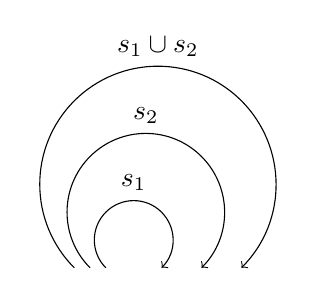
\begin{tikzpicture}
\path (0, 0) node (obj) {$\bigstar$};
\draw[->] (-0.2, 0) arc[radius=5mm, start angle=225, end angle=-45] node[pos=0.5, above]{$s_1$};
\draw[->] (-0.4, 0) arc[radius=10mm, start angle=225, end angle=-45] node[pos=0.5, above]{$s_2$};
\draw[->] (-0.6, 0) arc[radius=15mm, start angle=225, end angle=-45] node[pos=0.5, above]{$s_1 \cup s_2$};
\end{tikzpicture}
\captionsetup{labelformat=empty}
\end{figure}

Next let us see the additive monoid for natural numbers. Every number $n$ can define an arrow:

\[
\bigstar \arrowto{n} \bigstar
\]

The arrow composition is addition. Since addition is associative, hence arrow composition is also associative. Zero, 0 defines the identity arrow. This is because 0 adds to any number equals to this number itself. Therefore, the additive monoid for natural numbers does form a category.

\begin{figure}[htbp]
\centering
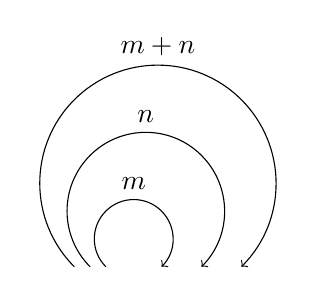
\begin{tikzpicture}
\path (0, 0) node (obj) {$\bigstar$};
\draw[->] (-0.2, 0) arc[radius=5mm, start angle=225, end angle=-45] node[pos=0.5, above]{$m$};
\draw[->] (-0.4, 0) arc[radius=10mm, start angle=225, end angle=-45] node[pos=0.5, above]{$n$};
\draw[->] (-0.6, 0) arc[radius=15mm, start angle=225, end angle=-45] node[pos=0.5, above]{$m + n$};
\end{tikzpicture}
\captionsetup{labelformat=empty}
\end{figure}


\item {In chapter 1, we introduced Peano's axioms for natural numbers and isomorphic structures to Peano arithmetic, like the linked-list etc. They can be described in categories. This was found by German mathematician Richard Dedekind although the category theory was not established by his time. We named this category as Peano category, denoted as $\pmb{Pno}$. The objects in this category is $(A, f, z)$, where $A$ is a set, for example natural numbers $N$; $f: A \to A$ is a successor function. It is $succ$ for natural numbers; $z \in A$ is the starting element, it is zero for natural numbers. Given any two Peano objects $(A, f, z)$ and $(B, g, c)$, define the morphism from $A$ to $B$ as:

\[
A \arrowto{\phi} B
\]

It satisfies:

\[
\phi \circ f = g \circ \phi \quad \text{and} \quad \phi(z) = c
\]

Verify that $\pmb{Pno}$ is a category.}

An object in Peano category is a tuple of $(A, f, z)$. An arrow is a map $\phi$ that preserve the tuple structure. Arrow composition is function composition:

\[ \begin{array}{l}
A \arrowto{\phi} B \arrowto{\psi} C \\
A \arrowto{\psi \circ \phi} C
\end{array}\]

Because function composition is associative, hence arrow composition is associative. For identity arrow:

\[
A \arrowto{id_A} A
\]

It satisfies $id_A(z) = z$, and $id_A \circ f = f \circ id_A$.

Obviously, the tuple $(\pmb{N}, succ, 0)$ is an object in Peano category. It's interesting that, for every object $(A, f, z)$ in Peano category, there is a unique arrow:

\[
(\pmb{N}, succ, 0) \arrowto{\sigma} (A, f, z)
\]

where:

\[
\sigma(n) = f^n(z)
\]

which maps any natural number $n$ to the result of applying $f$ to $z$ for $n$ times.

\item {For the list functor, define the arrow map with $foldr$.}

It's about to define list map with $foldr$ essentially:

\[
fmap\ f = foldr\ f\ Nil
\]

\item {Verify that the composition of maybe functor and list functor $\mathbf{Maybe} \circ \mathbf{List}$ and $\mathbf{List} \circ \mathbf{Maybe}$ are all functors.}

We only prove $\mathbf{Maybe} \circ \mathbf{List}$ is a functor. The other proof is similar. Any object $A$ is sent to $\mathbf{Maybe} (\mathbf{List}\ A)$. For arrows, let us first see the case of identity arrow:

\bre
(\mathbf{Maybe} \circ \mathbf{List})\ id & = & \mathbf{Maybe} (\mathbf{List}\ id) & \text{functor composition} \\
 & = & \mathbf{Maybe}\ id & \text{identity arrow for list functor} \\
 & = & id & \text{identity arrow for maybe functor} \\
\ere

Next is about arrow composition:

\bre
(\mathbf{Maybe} \circ \mathbf{List})\ (f \circ g) & = & \mathbf{Maybe} (\mathbf{List}\ (f \circ g)) & \text{functor composition} \\
 & = & \mathbf{Maybe} ((\mathbf{List}\ f) \circ (\mathbf{List}\ g)) & \text{composition for list functor} \\
 & = & (\mathbf{Maybe}\ (\mathbf{List}\ f)) \circ (\mathbf{Maybe}\ (\mathbf{List}\ g)) & \text{composition for maybe functor} \\
 & = & ((\mathbf{Maybe} \circ \mathbf{List})\ f) \circ ((\mathbf{Maybe} \circ \mathbf{List})\ g) & \text{functor composition} \\
\ere

\item {Proof that the composition for any functors $\mathbf{G} \circ \mathbf{F}$ is still a functor.}

Similar to previous exercise, we need prove functor composition satisfies identity arrow and arrow composition. First for identity arrow:

\bre
(\mathbf{G} \circ \mathbf{F})\ id & = & \mathbf{G} (\mathbf{F}\ id) & \text{functor composition} \\
 & = & \mathbf{G}\ id & \text{identity arrow for functor $\mathbf{F}$} \\
 & = & id & \text{identity arrow for functor $\mathbf{G}$} \\
\ere

Then for arrow composition:

\bre
(\mathbf{G} \circ \mathbf{F})\ (\phi \circ \psi) & = & \mathbf{G} (\mathbf{F}\ (\phi \circ \psi)) & \text{functor composition} \\
 & = & \mathbf{G} ((\mathbf{F}\ \phi) \circ (\mathbf{F}\ \psi)) & \text{arrow composition for functor $\mathbf{F}$} \\
 & = & (\mathbf{G}\ (\mathbf{F}\ \phi)) \circ (\mathbf{G}\ (\mathbf{F}\ \psi)) & \text{arrow composition for functor $\mathbf{G}$} \\
 & = & ((\mathbf{G} \circ \mathbf{F})\ \phi) \circ ((\mathbf{G} \circ \mathbf{F})\ \psi) & \text{functor composition} \\
\ere

\item {Give an example functor for preset.}

The functor for preset category is a monotone function.

\item {For the binary tree defined in chapter 2, define the functor for it.}

Consider an object $A$ in set total function category, the binary tree functor sends it to:

\lstset{language=Haskell, frame=none}
\begin{lstlisting}
data Tree A = Empty | Branch (Tree A) A (Tree A)
\end{lstlisting}

For arrow $A \arrowto{f} B$, the binary tree functor maps it to:

\bre
fmap\ f\ Empty & = & Empty \\
fmap\ f\ (Branch\ l\ x\ r) & = & Branch\ (fmap\ f\ l)\ (f\ x)\ (fmap\ f\ r) \\
\ere

Or we can use the $mapt$ defined in chapter 2:

\[
fmap = mapt
\]

\item{For any two objects in a poset, what is their product? what is their coproduct?}

In chapter 3, we mentioned any poset is a category, every element is the poset is an object, there is at most one arrow between two objects (the arrow exits if they have ordering relation). For two elements (objects) $a$ and $b$, if they have arrows both to the up and down stream, then:

\[
\text{meet}\ a \land b \quad \quad \quad \text{join}\ a \lor b
\]

is the

\[
\text{product} \quad \quad \quad \text{coproduct}
\]

for this pair of objects.

Where meet is the least upper bound (also called supremum) of the two objects, and join is the greatest lower bound (infimum) of them. In general, the join and meet of a subset of a partially ordered set need not exist, hence the product and coproduct of a poset need not exist too.

% https://en.wikipedia.org/wiki/Join_and_meet
%In mathematics, specifically order theory, the join and meet of a subset S of a partially ordered set P are respectively the supremum (least upper bound) of S, denoted ⋁S, and infimum (greatest lower bound) of S, denoted ⋀S. In general, the join and meet of a subset of a partially ordered set need not exist. Join and meet are dual to one another with respect to order inversion.

%\item {考虑集合范畴$\pmb{Set}$,积中的两个箭头$fst, snd$是右消去(epic)的么?和中的两个箭头$left, right$是左消去(monic)的么?}
\item {Prove the absorption law for coproduct, and verify the coproduct functor satisfies composition condition.}

The absorption law for coproduct states:

\[
[p, q] \circ (f + g) = [p \circ f, q \circ g]
\]

\begin{proof}
\blre
  & [p, q] \circ (f + g)  \\
= & [p, q] \circ [left \circ f, right \circ g] & \text{definition of $+$} \\
= & [[p, q] \circ (left \circ f), [p, q] \circ (right \circ g)] & \text{fusion law} \\
= & [[p, q] \circ left \circ f, [p, q] \circ right \circ g] & \text{associative} \\
= & [p \circ f, q \circ g] & \text{cancellation law} \\
\elre
\end{proof}

The composition condition for coproduct states:

\[
 (f + g) \circ (f' + g') = f \circ f' + g \circ g'
\]

\begin{proof}
Let $p = left \circ f$, and $q = right \circ g$

\blre
  & (f + g) \circ (f' + g') \\
= & [left \circ f, right \circ g] \circ (f' + g') & \text{definition of $+$} \\
= & [p, q] \circ (f' + g') & \text{substitute with $p, q$} \\
= & [p \circ f', q \circ g'] & \text{absorption law} \\
= & [left \circ f \circ f', right \circ g \circ g'] & \text{substitute $p, q$ back} \\
= & [left \circ (f \circ f'), right \circ (g \circ g')] & \text{associative law} \\
= & f \circ f' + g \circ g' & \text{reverse of $+$} \\
\elre
\end{proof}

\item{Prove that $swap$ satisfies the natural transformation condition $(g \times f) \circ swap = swap \circ (f \times g)$}

For $A \arrowto{f} C$ and $B \arrowto{g} D$, we need prove the below diagram commutes.

\begin{center}
\begin{tikzpicture}
  \matrix (m) [matrix of math nodes,
               row sep=3em, column sep=5em, minimum width=2em]{
     (A, B) & (B, A) \\
     (C, D) & (D, C) \\};
  \path[-stealth]
    (m-1-1) edge node [above] {$swap_{A, B}$} (m-1-2)
    (m-2-1) edge node [below] {$swap_{C, D}$} (m-2-2)
    (m-1-1) edge node [left] {$f \times g$} (m-2-1)
    (m-1-2) edge node [right] {$g \times f = swap\ f \times g$} (m-2-2);
\end{tikzpicture}
\end{center}

\begin{proof}
\blre
  & ((g \times f) \circ swap)\ (A, B) \\
= & (g \times f)\ (swap\ (A, B)) & \text{definition of composition} \\
= & (g \times f) \circ (B, A) & \text{definition of $swap$} \\
= & (g\ B, f\ A) & \text{product of arrows} \\
= & (D, C) & \text{definition of $g, f$} \\
= & swap\ (C, D) & \text{reverse of $swap$ definition} \\
= & swap\ (f\ A, g\ B) & \text{reverse of $f, g$ definition} \\
= & swap\ ((f \times g)\ (A, B)) & \text{product of arrow} \\
= & (swap \circ (f \times g))\ (A, B) & \text{reverse of composition} \\
\elre
\end{proof}

\item {Prove that the polymorphic function $length$ is a natural transformation. It is defined as the following:
\[
\begin{array}{l}
length : [A] \to Int \\
length\ [] = 0 \\
length\ (x:xs) = 1 + length\ xs
\end{array}
\]
}

For any object $A$, the arrow $length$ indexed by $A$ is:

\[
[A] \arrowto{length_A} \mathbf{K}_{Int}\ A
\]

where $\mathbf{K}_{Int}$ is constant functor. It sends every object to $Int$, and sends every arrow to identity arrow $id_{int}$. For arrow $A \arrowto{f} B$, we need prove below diagram commutes.

\begin{center}
\begin{tikzpicture}
  \matrix (m) [matrix of math nodes,
               row sep=3em, column sep=5em, minimum width=2em]{
     A & \lbrack A \rbrack & \mathbf{K}_{Int}\ A \\
     B & \lbrack B \rbrack & \mathbf{K}_{Int}\ B \\};
  \path[-stealth]
    (m-1-1) edge node [left] {$f$} (m-2-1)
    % square
    (m-1-2) edge node [above] {$length_A$} (m-1-3)
    (m-2-2) edge node [below] {$length_B$} (m-2-3)
    (m-1-2) edge node [left] {$\mathbf{List}(f)$} (m-2-2)
    (m-1-3) edge node [right] {$\mathbf{K}_{Int}(f)$} (m-2-3);
\end{tikzpicture}
\end{center}

From the definition of constant functor, this diagram is equivalent to:

\begin{center}
\begin{tikzpicture}
  \matrix (m) [matrix of math nodes,
               row sep=3em, column sep=5em, minimum width=2em]{
     A & \lbrack A \rbrack & Int \\
     B & \lbrack B \rbrack & Int \\};
  \path[-stealth]
    (m-1-1) edge node [left] {$f$} (m-2-1)
    % square
    (m-1-2) edge node [above] {$length_A$} (m-1-3)
    (m-2-2) edge node [below] {$length_B$} (m-2-3)
    (m-1-2) edge node [left] {$\mathbf{List}(f)$} (m-2-2)
    (m-1-3) edge node [right] {$id$} (m-2-3);
\end{tikzpicture}
\end{center}

We are about to prove:

\[
id \circ length_{A} = length_{B} \circ \mathbf{List}(f)
\]

Which means: $length_{A} = length_{B} \circ \mathbf{List}(f)$


\begin{proof}
Use mathematical induction, we first consider the empty list case:

\blre
  & length_B \circ \mathbf{List}(f) [] \\
= & length_B [] & \text{definition of list functor} \\
= & 0 & \text{definition of $length$} \\
= & length_A\ [] & \text{reverse of $length$ definition}
\elre

Next suppose $length_B \circ \mathbf{List}(f)\ as = length_A\ as$ holds, we have:

\blre
  & length_B \circ \mathbf{List}(f) (a:as) \\
= & length_B\ (f(a) : \mathbf{List}(f)\ as) & \text{definition of list functor} \\
= & 1 + length_B\ (\mathbf{List}(f)\ as) & \text{definition of $length$} \\
= & 1 + length_B\ \circ \mathbf{List}(f)\ as & \text{arrow composition} \\
= & 1 + length_A\ as & \text{induction assumption} \\
= & length_A\ (a:as) & \text{reverse of $length$ definition}
\elre
\end{proof}

\item {Natural transformation is composable. Consider two natural transformations $\mathbf{F} \arrowto{\phi} \mathbf{G}$ and $\mathbf{G} \arrowto{\psi} \mathbf{H}$. For any arrow $A \arrowto{f} B$, draw the diagram for their composition, and list the commutative condition.}

\begin{center}
\begin{tikzpicture}
  \matrix (m) [matrix of math nodes,
               row sep=3em, column sep=5em, minimum width=2em]{
     \mathbf{F}A & \mathbf{G}A & \mathbf{H}A \\
     \mathbf{F}B & \mathbf{G}B & \mathbf{H}B \\};
  \path[-stealth]
    (m-1-1) edge node [left] {$\mathbf{F}(f)$} (m-2-1)
    (m-1-1) edge node [above] {$\phi_A$} (m-1-2)
    (m-2-1) edge node [below] {$\phi_B$} (m-2-2)
    (m-1-2) edge node [above] {$\psi_A$} (m-1-3)
    (m-2-2) edge node [below] {$\psi_B$} (m-2-3)
    (m-1-2) edge node [left] {$\mathbf{G}(f)$} (m-2-2)
    (m-1-3) edge node [right] {$\mathbf{H}(f)$} (m-2-3);
\end{tikzpicture}
\end{center}

The commutative condition is:

\[
\mathbf{H}(f) \circ (\psi_A \circ \phi_A) = (\psi_B \circ \phi_B) \circ \mathbf{F} (f)
\]

\item{In the poset example, we say if there exists the minimum (or the maximum) element, then the minimum (or the maximum) is the initial object (or the final object). Consider the category of all posets $\pmb{Poset}$, if there exists the initial object, what is it? If there exists the final object, what is it?}

For the $\pmb{Poset}$ category, the objects are posets, the arrows are monotone functions. For two posets $P, Q$, arrow $P \arrowto{h} Q$ means for any two ordered elements $a \leq b$ in $P$, $h(a) \leq h(b)$ holds.

The initial object in this category is the empty poset $0 = \varnothing$. There is unique arrow from it to any poset $P$:

\[
\varnothing \longrightarrow P
\]

The final object is the singleton poset $1 = \{\bigstar\}$, the order relationship is $R = \{(\bigstar, \bigstar)\}$, i.e. $\bigstar \leq \bigstar$. From any poset $P$, there is unique arrow to 1:

\bre
P & \longrightarrow & \{\bigstar\} \\
p & \mapsto & \bigstar
\ere

\item{In the Peano category $\pmb{Pno}$ (see exercise 2 in section 1), what is the initial object in form $(A, f, z)$? What is the final object?}

The initial object is $(\pmb{N}, succ, 0)$. There is unique arrow from it to any object:

\[
(\pmb{N}, succ, 0) \arrowto{\sigma} (A, f, z): \sigma(n) = f^n(z)
\]

The final object is a singleton $1 = (\{\bigstar\}, \bigstar, id)$. There is unique arrow from any object $(A, f, z)$ to the final object:

\[
(A, f, z) \arrowto{\sigma} 1 : \sigma(a) = \bigstar
\]

\item{Verify that $\pmb{Exp}$ is a category. What is the $id$ arrow and arrow composition in it?}

Let us first verify the $id$ arrow $h \arrowto{id} h$, such that the following diagram commutes:

\begin{center}
\begin{tikzpicture}
  \matrix (m) [matrix of math nodes,
               row sep=3em, column sep=5em, minimum width=2em]{
     A & A \times B & \\
     A & A \times B & C \\};
  \path[-stealth]
    (m-1-1) edge node [left] {$id_A$} (m-2-1)
    (m-1-2) edge node [left] {$id_A \times id_B$} (m-2-2)
    (m-1-2) edge node [above] {$h$} (m-2-3)
    (m-2-2) edge node [below] {$h$} (m-2-3);
\end{tikzpicture}
\end{center}

Next is the arrow composition:

The composition of $h \arrowto{i} k$ and $k \arrowto{j} m$ is $j \circ i$ such that below diagram commutes:

\begin{center}
\begin{tikzpicture}
  \matrix (m) [matrix of math nodes,
               row sep=3em, column sep=5em, minimum width=2em]{
     A & A \times B & \\
     D & D \times B & C \\
     E & E \times B & \\};
  \path[-stealth]
    (m-1-1) edge node [left] {$f$} (m-2-1)
    (m-2-1) edge node [left] {$g$} (m-3-1)
    (m-1-2) edge node [left] {$f \times id_B$} (m-2-2)
    (m-2-2) edge node [left] {$g \times id_B$} (m-3-2)
    (m-1-2) edge node [above] {$h$} (m-2-3)
    (m-2-2) edge node [above] {$k$} (m-2-3)
    (m-3-2) edge node [below] {$m$} (m-2-3);
\end{tikzpicture}
\end{center}

For arrow $h \arrowto{j} k$, it means $id_k \circ j = j = j \circ id_h$ holds. And the associative law hold for any three arrows.

\item{In the reflection law $curry\ apply = id$, what is the subscript of the $id$ arrow? Please prove it with another method.}

The subscript of the $id$ arrow is the type of the binary arrow: $A \times B \to C$.

\begin{proof}
\blre
  & curry \circ apply\ f\ a\ b \\
= & curry\ (apply\ f)\ a\ b & \text{definition of composition} \\
= & (apply\ f)\ (a, b) & \text{definition of $curry$}\\
= & f(a, b) & \text{definition of $apply$} \\
= & id_{A \times B \to C}\ f(a, b)
\elre
\end{proof}

\item{We define the equation
\[
(curry\ f) \circ g = curry(f \circ (g \times id))
\]
as the fusion law for Currying. Draw the diagram and prove it.}

\begin{center}
\begin{tikzpicture}
  \matrix (m) [matrix of math nodes,
               row sep=3em, column sep=5em, minimum width=2em]{
     D & D \times B & \\
     A & A \times B & \\
     C^B & C^B \times B & C \\};
  \path[-stealth]
    (m-1-1) edge node [left] {$g$} (m-2-1)
    (m-2-1) edge node [left] {$curry\ f$} (m-3-1)
    (m-1-2) edge node [left] {$g \times id$} (m-2-2)
    (m-1-2) edge [bend right] node {} (m-3-2)
    (m-1-2) edge node [above] {$f \circ (g \times id)$} (m-3-3)
    (m-2-2) edge node [above] {$f$} (m-3-3)
    (m-3-2) edge node [below] {$apply$} (m-3-3);
\end{tikzpicture}
\end{center}

Observe the triangle of $D \times B$, $A \times B$, and $C$. We know the arrow of $D \times B \to C$ is $f \circ (g \times id)$.

According to the definition of exponentials and transpose arrow, we have:

\[
apply \circ (curry\ f) \circ g = f \circ (g \times id)
\]

According to the universal property of $curry$ and $apply$:

\[
(curry\ f) \circ g = curry (f \circ (g \times id))
\]

\item{Draw the diagram to illustrate the reverse element axiom for group.}

The reverse element axiom can be formalized as: $m \circ (id, i) = m \circ (i, id) = e$

\begin{center}
\begin{tikzpicture}
  \matrix (m) [matrix of math nodes,
               row sep=3em, column sep=5em, minimum width=2em]{
     G & G \times G & G \\
     1 & G & 1 \\};
  \path[-stealth]
    (m-1-1) edge node [above] {$(id, i)$} (m-1-2)
    (m-1-3) edge node [above] {$(i, id)$} (m-1-2)
    (m-1-1) edge node [left] {} (m-2-1)
    (m-1-2) edge node [left] {$m$} (m-2-2)
    (m-1-3) edge node [left] {} (m-2-3)
    (m-2-1) edge node [above] {$e$} (m-2-2)
    (m-2-3) edge node [above] {$e$} (m-2-2);
\end{tikzpicture}
\end{center}

\item{Let $p$ be a prime. Use the F-algebra to define the $\alpha$ arrow for the multiplicative group for integers modulo $p$ (refer to the previous chapter for the definition of this group).}

According to the $\alpha$ arrow defined for group:

\[
\mathbf{F} A \arrowto{\alpha = e + m +i} A
\]

The multiplicative group for integers modulo $p$ is defined as:

\bre
e\ () & = & 1 & \text{1 is the unit} \\
m(a, b) & = & ab \bmod p & \text{multiplication modulo $p$} \\
i(a) & = & a^{p-2} \bmod p & \text{Fermat's little theorem $a^{p-1} \equiv 1 \mod p$} \\
\ere

\item{Define F-algebra for ring (refer to the previous chapter for definition of ring).}

The algebraic structure of ring contains three parts:
\begin{enumerate}[i]
\item Carrier object $R$, the set that carries the algebraic structure of ring;
\item Polynomial functor $\mathbf{F}A = 1 + 1 + A \times A + A \times A + A$;
\item Arrow $\mathbf{F}A \arrowto{\alpha = z + e + p + m + n} A$, consists of the unit of addition $z$, the unit of multiplication $e$, addition $p$, multiplication $m$, and negation $n$.
\end{enumerate}

These define the $F$-algebra $(R, \alpha)$ for ring. When the carrier object is integers for example, the ring is defined as below under standard arithmetic:

\[\begin{array}{l}
z\ () = 0 \\
e\ () = 1 \\
p(a, b) = a + b \\
m(a, b) = ab \\
n(a) = -a \\
\end{array}\]

\item{What is the $id$ arrow for F-algebra category? What is the arrow composition?}

The $id$ arrow is the homomorphism from $F$-algebra $(A, \alpha)$ to itself. The arrow composition is the composition of $F$-morphisms. The arrow between carrier object $A \arrowto{f} B \arrowto{g} C$ makes the following diagram commute:

\begin{center}
\begin{tikzpicture}
  \matrix (m) [matrix of math nodes,
               row sep=3em, column sep=5em, minimum width=2em]{
     \mathbf{F} A & \mathbf{F} B & \mathbf{F} C \\
     A & B & C \\};
  \path[-stealth]
    (m-1-1) edge node [left] {$\alpha$} (m-2-1)
    (m-1-2) edge node [left] {$\beta$} (m-2-2)
    (m-1-3) edge node [left] {$\gamma$} (m-2-3)
    (m-1-1) edge node [above] {$\mathbf{F}(f)$} (m-1-2)
    (m-1-2) edge node [above] {$\mathbf{F}(g)$} (m-1-3)
    (m-2-1) edge node [below] {$f$} (m-2-2)
    (m-2-2) edge node [below] {$g$} (m-2-3);
\end{tikzpicture}
\end{center}

\[
  g \circ f \circ \alpha = \gamma \circ \mathbf{F}(g) \circ \mathbf{F}(f) = \gamma \circ \mathbf{F}(g \circ f)
\]

\item{Someone write the natural number like functor as the below recursive form. What do you think about it?
\begin{lstlisting}
data NatF A = ZeroF | SuccF (NatF A)
\end{lstlisting}
}

No, such definition does not work. Consider carrier object $A$, Functor $\mathbf{NatF}$ is recursive, it does not send $A$ to a determined object. In fact, we expect it is mapped to a object in Peano category $(A, f, z)$.

\item{We can define an $\alpha$ arrow for $\mathbf{NatF} Int \to Int$, named $eval$:
\[
\begin{array}{l}
eval : \mathbf{NatF} Int \to Int \\
eval\ ZeroF = 0 \\
eval\ (SuccF\ n) = n + 1 \\
\end{array}
\]
We can recursively substitute $A' = \mathbf{NatF} A$ to functor $\mathbf{NatF}$ by $n$ times. We denote the functor obtained as $\mathbf{NatF}^n A$. Can we define the following $\alpha$ arrow?
\[
\begin{array}{l}
eval : \mathbf{NatF}^n Int \to Int \\
\end{array}
\]
}

\bre
eval & : &\mathbf{NatF}^n Int \to Int \\
eval\ ZeroF & = & 0 & \text{$ZeroF$ is an object of $\mathbf{NatF}^n Int$}\\
eval\ (SuccF\ ZeroF) & = & 1 & \text{$ZeroF$ is an object of $\mathbf{NatF}^{n-1} Int$}\\
eval\ (SuccF\ (SuccF\ ZeroF)) & = & 2 & \text{$ZeroF$ is an object of $\mathbf{NatF}^{n-2} Int$}\\
... \\
eval\ (SuccF^{n-1}\ ZeroF) & = & n - 1 & \text{$ZeroF$ is an object of $\mathbf{NatF} Int$}\\
eval\ (SuccF^n\ m) & = & m + n \\
\ere

\item{For the binary tree functor $\mathbf{TreeF}\ A\ B$, fix $A$, use the fixed point to prove that $(\mathbf{Tree}\ A, [nil, branch])$ is the initial algebra}

Let $B' = \mathbf{TreeF}\ A\ B$. We recursively apply to itself, and call this result as $\mathbf{Fix}\ (\mathbf{TreeF}\ A)$.

\[
\resizebox{\textwidth}{!}{\ensuremath{
\begin{array}{rcll}
\mathbf{Fix}\ (\mathbf{TreeF}\ A) & = & \mathbf{TreeF}\ A\ (\mathbf{Fix}\ (\mathbf{TreeF}\ A)) & \text{definition of fixed point} \\
 & = & \mathbf{TreeF}\ A\ (\mathbf{TreeF}\ A (...)) & \text{expand} \\
 & = & NilF | BrF\ A\ (\mathbf{TreeF}\ A\ (...))\ (\mathbf{TreeF}\ A\ (...)) & \text{definition of binary tree functor} \\
 & = & NilF | BrF\ A\ (\mathbf{Fix}\ (\mathbf{TreeF}\ A))\ (\mathbf{Fix}\ (\mathbf{TreeF}\ A)) & \text{reverse of fixed point} \\
\end{array}
}}
\]

Compare with the definition of $Tree A$:

\begin{lstlisting}
data Tree A = Nil | Br A (Tree A) (Tree A)
\end{lstlisting}

Hence $\mathbf{Tree}\ A = \mathbf{Fix}\ (\mathbf{TreeF}\ A)$. The initial algebra is $(\mathbf{Tree}\ A, [nil, branch])$.

\end{enumerate}

\section{Fusion}

\begin{enumerate}
\item{Verify that folding from left can also be defined with $foldr$:
\[
foldl\ f\ z\ xs = foldr\ (b\ g\ a \mapsto g\ (f\ a\ b))\ id\ xs\ z
\]}

To make it easy, we rewrite it to:

\[\begin{array}{l}
foldl\ f\ z\ xs = foldr\ step\ id\ xs\ z \\
\text{where}: step\ x\ g\ a = g\ (f\ a\ x)
\end{array}\]

\blre
  & foldl\ f\ z\ [x_1, x_2, ..., x_n] \\
= & (foldr\ step\ id\ [x_1, x_2, ..., x_n])\ z \\
= & (step\ x_1 (step\ x_2 ( ... (step\ x_n\ id))) ...)\ z \\
= & (step\ x_1 (step\ x_2 ( ... (a_n \mapsto id\ (f\ a_n\ x_n)))) ...)\ z \\
= & (step\ x_1 (step\ x_2 ( ...(a_{n-1} \mapsto (a_n \mapsto id\ (f\ a_n\ x_n))\ (f\ a_{n-1}\ x_{n-1}))))...)\ z \\
= & (a_1 \mapsto (a_2 \mapsto ( ... (a_n \mapsto id\ (f\ a_n\ x_n))\ (f\ a_{n-1}\ x_{n-1})) ... (f\ a_2\ x_2)) (f\ a_1\ x_1))\ z \\
= & (a_1 \mapsto (a_2 \mapsto ( ... (a_n \mapsto f\ a_n\ x_n)\ (f\ a_{n-1}\ x_{n-1})) ... )\ (f\ a_1\ x_1))\ z \\
= & (a_1 \mapsto (a_2 \mapsto (... (a_{n-1} \mapsto f\ (f\ a_{n-1}\ x_{n-1})\ x_n)\ ...))\ (f\ a_1\ x_1))\ z \\
= & (a_1 \mapsto f\ (f\ (...(f\ a_1\ x_1)\ x_2)\ ...)\ x_n)\ z \\
= & f\ (f\ (...(f\ z\ x_1)\ x_2)\ ...)\ x_n
\elre

We can further write $f$ as an infix of $\oplus$ to highlight the difference between $foldl$ and $foldr$:

\[
foldl\ \oplus\ f\ z = ((...(z \oplus x_1)\ \oplus x_2)...)\ \oplus x_n
\]

\item{Prove the below build...foldr forms hold:
\[
\begin{array}{l}
concat\ xss = build\ (f\ z \mapsto foldr\ (xs\ x \mapsto foldr\ f\ x\ xs)\ z\ xss) \\
map\ f\ xs = build\ (\oplus\ z \mapsto foldr\ (y\ ys \mapsto (f\ y) \oplus ys)\ z\ xs) \\
filter\ f\ xs = build\ (\oplus\ z \mapsto foldr\ (x\ xs' \mapsto
  \begin{cases}
     f(x): & x \oplus xs' \\
    \text{otherwise}: & xs' \\
  \end{cases})\ z\ xs) \\
repeat\ x = build\ (\oplus\ z \mapsto let\ r = x \oplus r\ in\ r) \\
\end{array}
\]
}

First for the list $concat$:

\begin{proof}
\blre
  & build\ (f\ z \mapsto foldr\ (xs\ x \mapsto foldr\ f\ x\ xs)\ z\ xss) \\
= & (f\ z \mapsto foldr\ (xs\ x \mapsto foldr\ f\ x\ xs)\ z\ xss)\ (:)\ [] & \text{definition of $build$} \\
= & foldr\ (xs\ x \mapsto foldr\ (:)\ x\ xs)\ []\ xss & \text{$\beta$-reduction} \\
= & foldr\ \doubleplus []\ xss & \text{concatenate two lists} \\
= & concat\ xss & \text{concatenate multiple lists} \\
\elre
\end{proof}

Next for list $map$

\begin{proof}
\blre
  & build\ (\oplus\ z \mapsto foldr\ (y\ ys \mapsto (f\ y) \oplus ys)\ z\ xs) \\
= & (\oplus\ z \mapsto foldr\ (y\ ys \mapsto (f\ y) \oplus ys)\ z\ xs)\ (:)\ [] & \text{definition of $build$} \\
= & foldr\ (y\ ys \mapsto f(y) : ys)\ []\ xs & \text{$\beta$-reduction} \\
= & foldr\ (x\ ys \mapsto f(x) : ys)\ []\ xs & \text{$\alpha$ transformation, change name} \\
= & map\ f\ xs & \text{definition of list map} \\
\elre
\end{proof}

Next for $filter$

\begin{proof}
\blre
  & build\ (\oplus\ z \mapsto foldr\ (x\ xs' \mapsto
  \begin{cases}
     f(x): & x \oplus xs' \\
    \text{otherwise}: & xs' \\
  \end{cases})\ z\ xs) \\
= & (\oplus\ z \mapsto foldr\ (x\ xs' \mapsto
  \begin{cases}
     f(x): & x \oplus xs' \\
    \text{otherwise}: & xs' \\
  \end{cases})\ z\ xs)\ (:)\ [] & \text{definition of $build$} \\
= & foldr\ (x\ xs' \mapsto
  \begin{cases}
     f(x): & x : xs' \\
    \text{otherwise}: & xs' \\
  \end{cases})\ []\ xs & \text{$\beta$-reduction} \\
= & filter\ f\ xs & \text{definition of filter} \\
\elre
\end{proof}

Last for $repeat$

\begin{proof}
\blre
  & build\ (\oplus\ z \mapsto let\ r = x \oplus r\ in\ r) \\
= & (\oplus\ z \mapsto let\ r = x \oplus r\ in\ r)\ (:)\ [] & \text{definition of $build$} \\
= & (let\ r = x : r\ in\ r) & \text{$\beta$-reduction} \\
= & repeat\ x & \text{definition of repeat} \\
\elre
\end{proof}

\item{Simplify the quick sort algorithm.
\[
\begin{cases}
qsort\ [] = [] \\
qsort\ (x:xs) = qsort\ [a | a \in xs, a \leq x] \doubleplus [x] \doubleplus qsort\ [a | a \in xs, x < a] \\
\end{cases}\]
}

First, we can transform the ZF-expression to $filter$, and combine the two rounds of list filtering to one pass:

\[
\begin{cases}
qsort\ [] & = [] \\
qsort\ (x:xs) & = qsort\ as \doubleplus [x] \doubleplus qsort\ bs \\
\end{cases}
\]

where:
\[\begin{array}{l}
(as, bs) = foldr\ h\ ([], [])\ xs \\
h\ y\ (as', bs') = \begin{cases}
               y \leq x : & (y:as', bs') \\
               \text{otherwise}: & (as', y:bs') \\
\end{cases} \\
\end{array}\]

Next we further simplify the list concatenation:

\blre
  & qsort\ as \doubleplus [x] \doubleplus qsort\ bs \\
= & qsort\ as \doubleplus (x : qsort\ bs) \\
= & foldr (:)\ (x : qsort\ bs) (qsort\ as)
\elre

\item{Verify the type constraint of fusion law with category theory. Hint: consider the type of the catamorphism.}

As shown in below diagram:

\begin{center}
\begin{tikzpicture}
  \matrix (m) [matrix of math nodes,
               row sep=3em, column sep=5em, minimum width=2em]{
     \mathbf{ListF} A\ \lbrack A \rbrack & \lbrack A \rbrack \\
     \mathbf{ListF} A\ B\ & B \\};
  \path[-stealth]
    (m-1-1) edge node [left] {$\mathbf{ListF} A(h)$} (m-2-1)
    (m-1-2) edge node [right] {$h = \lbb \alpha \rbb$} (m-2-2)
    (m-1-1) edge node [above] {$(:) + []$} (m-1-2)
    (m-2-1) edge node [below] {$\alpha = f + z$} (m-2-2);
\end{tikzpicture}
\end{center}

The catamorphism $\lbb \alpha \rbb$ is abstracted to build some algebraic structure from $\alpha$, i.e. $g\ \alpha$. Where $g$ accepts the $\alpha$ arrow of an $F$-algebra, generates result of $B$. The $\alpha$ arrow is the coproduct of $f : A \to B \to B$ and $z : 1 \to B$, that the type is:

\[
g : \forall A. (\forall B. (A \to B \to B) \to B \to B)
\]

The definition of build is $build(g) = g\ (:)\ []$. It applies $g$ to the $\alpha$ arrow of the initial algebra, and builds the object of the initial algebra, which is a list of $[A]$.

\[
build : \forall A. (\forall B. (A \to B \to B) \to B \to B) \to \mathbf{List}\ A
\]

\item{Use the fusion law to optimize the expression evaluation function:
\[
eval = sum \circ map\ (product \circ (map\ dec))
\]}

\[
\resizebox{\textwidth}{!}{\ensuremath{
\begin{array}{cll}
  & eval\ es \\
= & sum (map\ (product \circ (map\ dec))\ es) & \text{function composition} \\
  & \{ \text{$sum$ in fold, $map$ in build} \} \\
= & \pmb{foldr}\ (+)\ 0\ (\pmb{build}\ (\oplus\ z\ \mapsto foldr\ (t\ ts \mapsto (f\ t) \oplus ts)\ z\ es)) & \text{let $f = product \circ (map\ dec)$} \\
= & (\oplus\ z \mapsto foldr\ (t\ ts \mapsto (f\ t) \oplus ts)\ z\ es)\ (+)\ 0 & \text{fusion law} \\
= & foldr\ (t\ ts \mapsto (f\ t) + ts)\ 0\ es & \text{$\beta$-reduction} \\
\end{array}
}}
\]

Written in point-free form as:

\[
eval = foldr\ (t\ ts \mapsto (f\ t) + ts)\ 0
\]

Next we simplify the $product \circ (map\ dec)$ part

\[
\resizebox{\textwidth}{!}{\ensuremath{
\begin{array}{cll}
  & (product \circ (map\ dec))\ t \\
= & product\ (map\ dec\ t) & \text{function composition} \\
  & \{ \text{$product$ in fold, $map$ in build} \} \\
= & \pmb{foldr}\ (\times)\ 1\ (\pmb{build}\ (\oplus\ z \mapsto foldr\ (d\ ds \mapsto (dec\ d) \oplus ds)\ z\ t)) \\
= & (\oplus\ z \mapsto foldr (d\ ds \mapsto (dec\ d) \oplus ds)\ z\ t)\ (\times)\ 1 & \text{fusion law} \\
= & foldr\ (d\ ds \mapsto (dec\ d) \times ds)\ 1\ t & \text{$\beta$-reduction} \\
= & foldr\ ((\times) \circ fork\ (dec, id))\ 1\ t & \text{let $fork(f, g)\ x = (f\ x, g\ x)$} \\
\end{array}
}}
\]

Substitute this to $f$, we obtain the final simplified result:

\[
eval = foldr\ (t\ ts \mapsto (foldr\ ((\times) \circ fork\ (dec, id))\ 1\ t) + ts)\ 0
\]

\item{How to expand all expressions from left?}

When expand from left to right, there are three options for every digit $d$:

\begin{enumerate}
\item Insert nothing. It means append $d$ to the last factor of the last sub-expression of $e_i$. Combine $f_n \doubleplus [d]$ as a new factor. For example when $e_i$ is $1 + 2$, $d$ is 3, write 3 after $1 + 2$ without inserting any symbols, we obtain a new expression $1 + 23$;

\item Insert $\times$. It means we create a new factor $[d]$, then append it to the last sub-expression of $e_i$. Combine $t_m \doubleplus [[d]]$ as a new sub-expression. For the same $1 + 2$ example, we write 3 after it, put a $\times$ between 2 and 3, hence obtain a new sub-expression $1 + 2 \times 3$;

\item Insert +. It means we create a new sub-expression $[[d]]$, then append it to $e_i$ to obtain a new expression $e_i \doubleplus [[[d]]]$. For the same $1 + 2$ example, we write 3 after it, put a + between 2 and 3, hence obtain a new expression $1 + 2 + 3$.
\end{enumerate}

We need define the append function to add an element after a list:

\[
append\ x = foldr\ (:)\ [x]
\]

Then we define a function $onLast(f)$, which applies $f$ to the last element of a list:

\[\begin{array}{l}
onLast\ f = foldr\ h\ [] \\
\text{where}: \begin{cases}
  h\ x\ [] & = [(f\ x)] \\
  h\ x\ xs & = x : xs \\
\end{cases} \\
\end{array}\]

Then we implement the above three expansion options:

\lstset{frame = none}
\begin{lstlisting}
add d exp = [((append d) `onLast`) `onLast` exp,
             (append [d]) `onLast` exp,
             (append [[d]]) exp]
\end{lstlisting}

\item{The following definition converts expression to string:
\[
str = (join\ \text{``+''}) \circ (map\ ((join\ \text{``} \times \text{''}) \circ (map\ (show \circ dec))))
\]
Where $show$ converts number to string. Function $join(c, s)$ concatenates multiple strings $s$ with delimiter $c$. For example: $join($``\#''$, [$``abc'', ``def''$]) = $``abc\#def''. Use the fusion law to optimize $str$.
}

We defined $join(ws)$ in chapter 5. It insert space between every two strings. We can extract the space as a parameter to define $join(c, s)$:

\[
join\ c = foldr\ (w\ b \mapsto foldr\ (:)\ (c:b)\ w)\ []
\]

Observe the definition of $str$. It contains embedded $(join\ c) \circ (map\ f)$ as:

\[\begin{array}{l}
str = (join\ c) \circ (map\ f) \\
\text{where}: f = (join\ d) \circ (map\ g) \\
\end{array}\]

where $c =$ `+', $d =$ `$\times$', and $g = show \circ dec$. What we need is to simplify $(join\ c) \circ (map\ f)$.

\blre
  & (join\ c) \circ (map\ f)\ es \\
  & \{ \text{$join$ in fold, $map$ in build} \} \\
= & \pmb{foldr}\ (w\ b \mapsto foldr\ (:) (c:b)\ w)\ []\ (\pmb{build}\ (\oplus\ z \mapsto foldr\ (y\ ys \mapsto (f\ y) \oplus ys)\ z\ es)) \\
  & \{ \text{fusion law} \} \\
= & (\oplus\ z \mapsto foldr\ (y\ ys \mapsto (f\ y) \oplus ys)\ z\ es))\ (w\ b \mapsto foldr\ (:)\ (c:b)\ w)\ [] \\
  & \{ \text{$\beta$-reduction} \} \\
= & foldr\ (y\ ys \mapsto foldr\ (:)\ (c:ys)\ (f\ y))\ []\ es \\
\elre

Substitute the +, $\times$, and $show \circ dec$ in, we obtain the final result:

\blre
str & = & foldr\ (x\ xs \mapsto foldr\ (:)\ (`+':xs) ( \\
    &   & \quad foldr (y\ ys \mapsto foldr\ (:)\ (`\times':ys)\ (show \circ dec\ y))\ [])\ [] \\
\elre

\end{enumerate}

\section{Infinity}

\begin{enumerate}

\item{In chapter 1, we realized Fibonacci numbers by folding. How to define Fibonacci numbers as potential infinity with $iterate$?}

\[
F = (fst \circ unzip)\ (iterate\ ((m, n) \mapsto (n, m + n))\ (1, 1))
\]

For example $take\ 100\ F$ gives the first 100 Fibonacci numbers

\item{Define $iterate$ by folding.}

Consider the infinite stream $iterate\ f\ x$. After applying $f$ to each element, and prepend $x$ as the first one, we obtain this infinite stream again. Based on this fact, we can define it as:

\[
iterate\ f\ x = x : foldr (y\ ys \mapsto (f\ y):ys)\ []\ (iterate\ f\ x)
\]

For example:

\begin{lstlisting}
take 10 $ iter (+1) 0
[0,1,2,3,4,5,6,7,8,9]
\end{lstlisting} %$

\item{Use the definition of the fixed point in chapter 4, prove $Stream$ is the fixed point of $StreamF$.}

Let $A' = \mathbf{StreamF}\ E\ A$, then apply it to itself repeatedly. We call this result $\mathbf{Fix}\ (\mathbf{StreamF}\ E)$

\bre
\mathbf{Fix}\ (\mathbf{StreamF}\ E) & = &
    \mathbf{StreamF}\ E\ (\mathbf{Fix}\ (\mathbf{StreamF}\ E)) & \text{definition of fixed point} \\
 & = & \mathbf{StreamF}\ E\ (\mathbf{StreamF}\ E\ (...)) & \text{expand recursively} \\
 & = & \mathbf{Stream}\ E\ (\mathbf{Stream}\ E\ (...)) & \text{change name} \\
 & = & \mathbf{Stream}\ E & \text{reverse of $Stream$} \\
\ere

Therefore, $Stream$ is the fixed point of $StreamF$.

\item{Define $unfold$.}

We often use $Maybe$ to define the terminate condition:

\begin{lstlisting}
unfold :: (b -> Maybe (a, b)) -> (b -> [a])
unfold f b = case f b of
                Just (a, b') -> a : unfold f b'
                Nothing -> []
\end{lstlisting}

\item{The fundamental theorem of arithmetic states that, any integer greater than 1 can be unique represented as the product of prime numbers. Given a text $T$, and a string $W$, does any permutation of $W$ exist in $T$? Solve this programming puzzle with the fundamental theorem and the stream of prime numbers.}

Our idea is to map every unique character to a prime number, for example, a $\to$ 2, b $\to$ 3, c $\to$ 5, ... Given any string $W$, no matter it contains repeated characters or not, we can convert it to a product of prime numbers:

\[
F = \prod p_c , c \in W
\]

We call it the number theory finger print $F$ of string $W$. When $W$ is empty, we define its finger print as 1. Because multiplication of integers is commutative, the finger print is same for all permutations of $W$, and according to the fundamental theorem of arithmetic, the finger print is unique. We can develop an elegant solution based on this: First, we calculate $F$ of string $W$, then slide a window of length $|W|$ along $T$ from left to right. When start, we also need to compute the finger print within this window of $T$, and compare it with $F$. If they are equal, it means $T$ contains some permutation of $W$. Otherwise, we slide the window to the right by a character. We can easily compute the updated finger print value for this new window position: divide the product by the prime number of the character slides out, and multiply the prime number of the character slides in. Whenever the finger print equals to $F$, we find a permutation. In order to map different characters to prime numbers, we can use sieve of Eratosthenes to generate a series of prime numbers. Below is the example algorithm accordingly.

\begin{algorithmic}
\Function{contains?}{$W, T$}
  \State $P \gets ana \ era \ [2, 3, ...]$ \Comment{prime numbers}
  \If{$W = \phi$}
    \State \Return True
  \EndIf
  \If{$|T| < |W|$}
    \State \Return False
  \EndIf
  \State $\displaystyle m \gets \prod P_c, c \in W$
  \State $\displaystyle m' \gets \prod P_c, c \in T[1...|W|]$
  \For{$i \gets |W| + 1$ to $|T|$}
    \If{$m = m'$}
      \State \Return True
    \EndIf
    \State $m' \gets m' \times P_{T_i} / P_{T_{i - |W|}} $
  \EndFor
  \State \Return $m = m'$
\EndFunction
\end{algorithmic}

\item{We establish the 1-to-1 correspondence between the rooms and guests. For guest $i$ in group $j$, which room number should be assigned? Which guest in which group will live in room $k$?}

Use the convention to count from zero, and use pair $(i, j)$ to denote the $j$-th guest in the $i$-th group. Let us list the first several guests and their rooms:

%\begin{adjustbox}{max width=\textwidth}
\btab{c|c|c|c|c|c|c|c|c|c|c|c}
$(i, j)$ & (0, 0) & (0, 1) & (1, 0) & (2, 0) & (1, 1) & (0, 2) & (0, 3) & (1, 2) & (2, 1) & (3, 0) & ... \\
\hline
$k$ & 0 & 1 & 2 & 3 & 4 & 5 & 6 & 7 & 8 & 9 & ... \\
\hline
$i + j$ & 0 & 1 & 1 & 2 & 2 & 2 & 3 & 3 & 3 & 3 & ... \\
\etab
%\end{adjustbox}

Writing down the values $i+j$, we can find the pattern. There are 1 instance of number 0, 2 instances of number 1, 3 instances of number 2, 4 instances of number 3, ... They are exactly the triangle numbers found by Pythagoreans. Let $m = i + j$, there are total $\dfrac{m(m + 1)}{2}$ grid points along the diagonals on the left-bottom side of a given grid.

For the diagonal where this point belongs to, if $m$ is odd, then the room number increases along the left up direction,  $i$ increases, and $j$ decreases; if $m$ is even, then the direction is right-bottom. Summarize the two cases gives the following result:

\[
k = \dfrac{m(m + 1)}{2} + \begin{cases} m - j: \text{$m$ is odd} \\
j: \text{$m$ is even} \\
\end{cases}
\]

Further, we can use $(-1)^m$ to simplify the conditions:

\[
k = \dfrac{m(m + 2) + (-1)^m (2j - m)}{2}
\]

\item{For Hilbert's Grand hotel, there are multiple solutions for the problem on the third day. Can you give a different numbering scheme based on the cover page of the book {\em Proof without word}?}

\begin{figure}[htbp]
\centering
\begin{tikzpicture}
  \draw[step=1, very thin, gray] (0, 0) grid (5, 5);
  \draw[->] (-0.25, 0) -- (6, 0) coordinate (x axis);
  \draw[->] (0, -0.25) -- (0, 6) coordinate (y axis);
  \foreach \x in {0, 1, 2, 3, 4, 5}
    \path (\x, -0.25) node[left] {\x};
  \foreach \y in {1, 2, 3, 4, 5}
    \path (-0.25, \y) node[below] {\y};
  \foreach \i / \x / \y in {0/0/0, 1/1/0, 2/1/1, 3/0/1, 4/0/2, 5/1/2, 6/2/2, 7/2/1, 8/2/0, 9/3/0, 10/3/1}{
    \path (\x, \y) coordinate (N\i);
    \fill (N\i) circle (1pt) node[above right=3pt of N\i] {\i};
  }
  \foreach \i in {0,...,9} {
    \pgfmathsetmacro{\j}{\i+1}
    \draw[-latex, thick] (N\i) to (N\j);
  }
\end{tikzpicture}
\caption{Another numbering scheme for infinity of infinity}
\label{fig:NNtoN2}
\end{figure}

As shown in figure \ref{fig:NNtoN2}, we count along the gnomon shaped path. There are odd number of grid points along every gnomon.

\item{Let $x = 0.9999....$, then $10x = 9.9999...$, subtract them gives $10x - x = 9$. Solving this equation gives $x = 1$. Hence $1 = 0.9999...$. Is this proof correct?}

Yes, it's correct.

\item{Light a candle between two opposite mirrors, what image can you see? Is it potential or actual infinity?}

The candle image reflects between the two mirrors endlessly, generates infinite many images. If we consider the speed of light is limited, then it is potential infinity from physics viewpoint.

\end{enumerate}

\section{Paradox}

\begin{enumerate}
\item{We can define numbers in natural language. For example ``the maximum of two digits number'' defines 99. Define a set containing all numbers that cannot be described within 20 words. Consider such an element: ``The minimum number that cannot be described within 20 words''. Is it a member of this set?}

This is an instance of Russell's paradox. Whether it is a member, all lead to contradiction.

\item{``The only constant is change'' said by Heraclitus. Is this Russell's paradox?}

Yes, this is an instance of Russell's paradox.

\item{Is the quote saying by Socrates (the beginning of chapter 7) Russell's paradox?}

Yes, it is an instance of Russell's paradox.

\item{Translate Fermat's last theorem into a TNT string.}

We need define power operation first.

\[\begin{cases}
\forall a: e(a, 0) = S0 & \text{0-th power is 1} \\
\forall a: \forall b: e(a, Sb) = a \cdot e(a, b) & \text{recursion} \\
\end{cases}\]

We can then define Fermat's last theorem atop it.

\[
\forall d: \lnot \exists a: \exists b: \exists c: \lnot (d = 0 \lor d = S0 \lor d = SS0) \to e(a, d) + e(b, d) = e(c, d)
\]

\item{Prove the associative law of addition with TNT reasoning rules.}

Surprisingly, we can prove every theorem below:

\bre
a + b + 0 & = & a + (b + 0) \\
a + b + S0 & = & a + (b + S0) \\
a + b + SS0 & = & a + (b + SS0) \\
... \\
\ere

For example:

\bre
a + b + 0 = a + b = a + (b + 0)
\ere

And:

\bre
a + b + SS0 & = & SS(a + b + 0) \\
 & = & SS(a + b) \\
 & = & a + SSb \\
 & = & a + (b + SS0) \\
\ere

However, we cannot prove: $\forall c: a + b + c = a + (b + c)$.

To do that, we has to introduce mathematical induction.

\item{Prove that $\forall a: (0 + a) = a$ with the newly added rule of induction.}

First for the case of 0:

\[
0 + 0 = 0
\]

Next suppose $(0 + a) = a$ holds, we have:

\bre
(0 + Sa) & = & S(0 + a) & \text{axiom 3} \\
  & = & Sa & \text{induction hypothesis} \\
\ere

From the rule of induction, we obtain: $\forall a: (0 + a) = a$

\end{enumerate}

\ifx\wholebook\relax \else
\begin{thebibliography}{99}

\bibitem{Lockhart2012}
Paul Lockhart. ``Measurement''. Belknap Press: An Imprint of Harvard University Press; Reprint edition 2014, ISBN: 978-0674284388

\end{thebibliography}

\expandafter\enddocument
%\end{document}

\fi
